\section{Integration at the FileDownload Level}

\subsection{Changes to the FileDownload agent}

\subsection{Setup and test}
The prototype was tested on ANSE's testbed (Figure \ref{fig:testbed}) using 
two sites: T2\_ANSE\_Amsterdam and T2\_ANSE\_Geneva. These sites consist of two
 servers each: a PhEDEx server and a dedicated storage server for that particular 
 PhEDEx instance. Each of the two storage servers consist of dual 8 core CPUs 
 (with HT), 64GB of RAM and 2 LSI controllers which manage 8 SSDs each. We created 
 two RAID-0 partitions of 4 SSDs each on every LSI controller. Since the tests are write 
 intensive and were scheduled to run for around 24 hours, we decided to only use 
 1 controller, in order to minimize the negative effects on the lifetime of the disks.

The two sites were connected via a high speed 40Gbps link. On this link we could create
static virtual circuits and for the purposes of our test we decided to create two new
circuits of 10 Gbps each.

One of these circuits was used to model a shared link in which PhEDEx had to compete 
with other traffic. This background traffic was generated by Iperf and consisted of a 
continuous stream of UDP packets at 5Gbps . The other circuit served as the dedicated
link.

Monitoring was done with MonALISA\footnote{MONitoring Agents using Large
 Integrated Services Architecture (monalisa.cern.ch) } and the PhEDEx tool itself.

The main purpose of this test wasn't to show that we can saturate a 10Gbps link with
PhEDEX (although we came close with just 1 controller), but that a PhEDEx instance 
is able to switch to using a new path in a transparent manner for the other instances
and with no down time. 

The first part of the test consisted of a 10 hour run with PhEDEx transfers on the 
shared link. After this time, PhEDEx switched to using the dedicated circuit and
continued transfers for another 10 hours.

We set up PhEDEx to run a single 450 GB transfer job at a time, each one 
comprising of 30 files of 15 GB each. 

\begin{figure}[h]
  \centering
  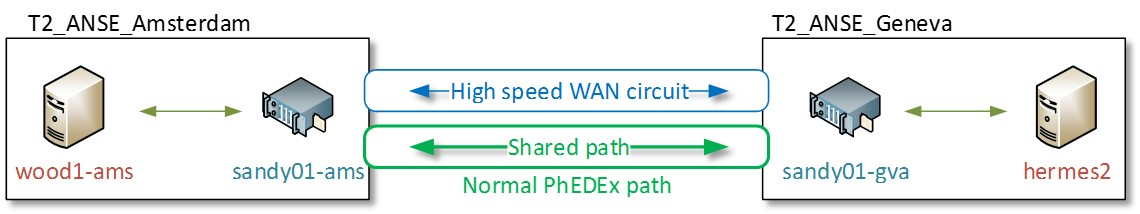
\includegraphics[width=0.95\textwidth]{FileDownload_ANSE_Testbed}
  \caption{Diagram of the testbed used by the prototype}
  \label{fig:testbed}
\end{figure} 


\subsection{Results}

The results of the first half of the test are shown in  (Figure \ref{fig:shared_transfers}).
A quick glance at this plot, shows that the 10 Gbps link was saturated by the two
competing transfers. Between 23:00 and 0:00 (beginning of the plot) and 
10:00 and 11:00 (end of the plot), only UDP traffic was sent across the network, 
running at a steady 5 Gbps. This effectively leaves only 5 Gbps of PhEDEx traffic.
PhEDEx transfers start around 0:00 and quickly saturate the 10 Gbps. 
The seesaw look of this plot is due to the fact that PhEDEx has a delay
between finishing one job and starting the next. This is due to various factors:
 pre/post validation, preparation of copyjobs or even time spent by the backend itself 
 before actually launching a transfer. Because of these delays, the average 
 rates reported by PhEDEx will always be lower than the average rates of each
 individual transfer job. Nevertheless we get average transfer rates of 9.5 Gbps for the
 whole link and consequently 4.5 Gbps for PhEDEx transfers (10\% penalty from
 gap between jobs).

\begin{figure}[h]
  \centering
  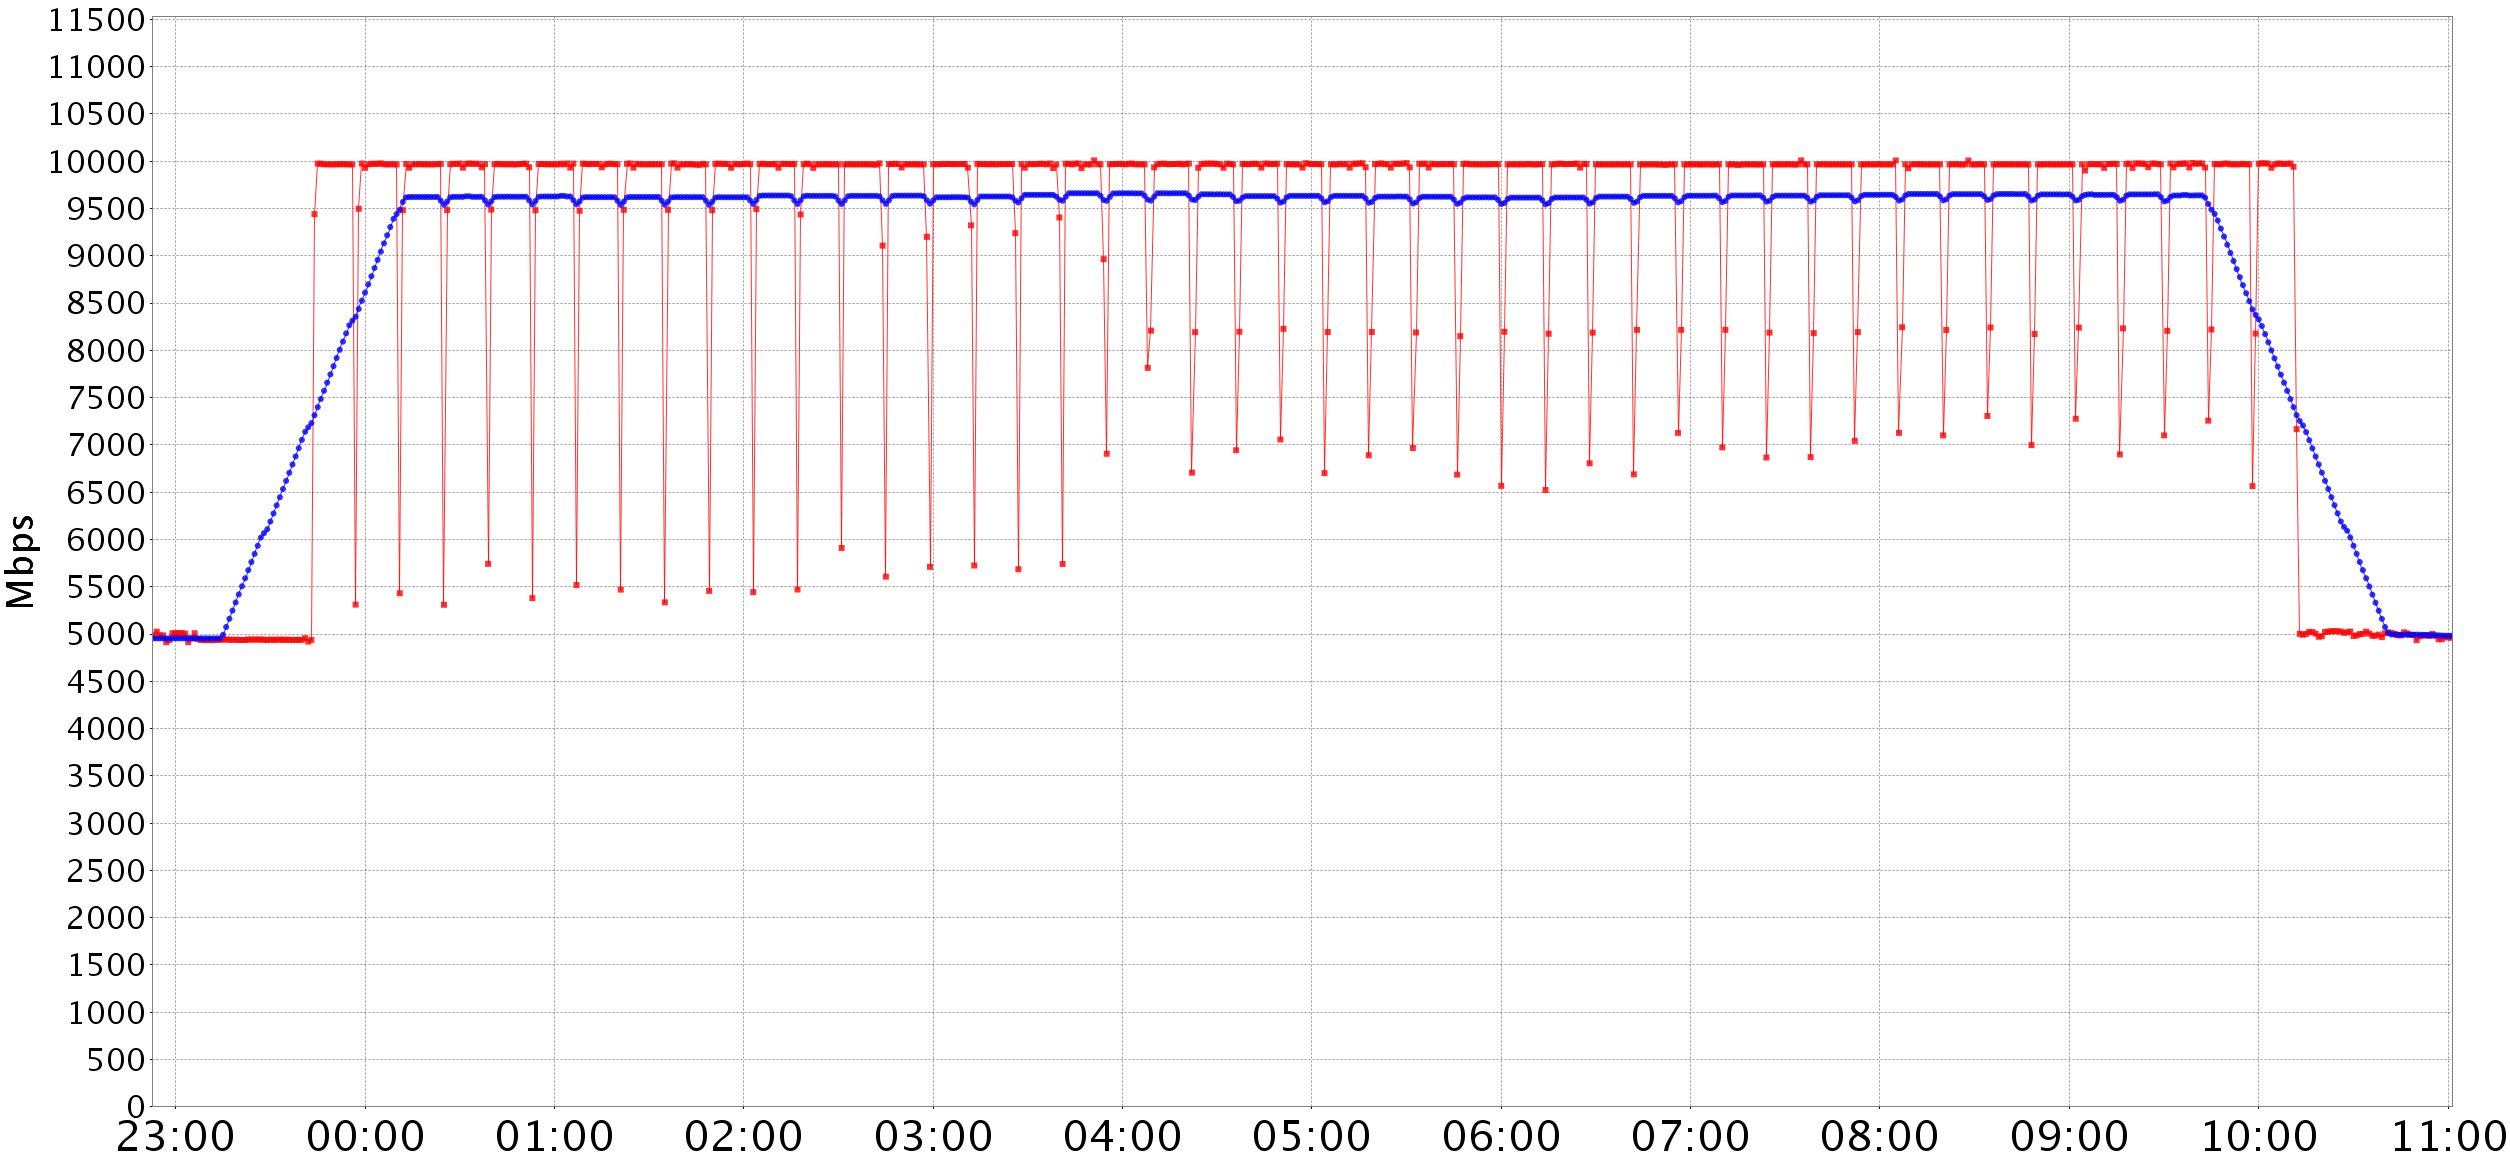
\includegraphics[width=0.95\textwidth]{FileDownload_Shared_path.png}
  \caption{PhEDEx transfers on the shared path - competing with 5Gbps UDP traffic}
  \label{fig:shared_transfers}
\end{figure} 

Around 10:00 PhEDEx switches to using the dedicated link. The results of the 
second half of the test are shown in Figure \ref{fig:solo_transfers}.

Although most of the time we are able to saturate the 10Gbps link with PhEDEx 
traffic alone we sometimes see dips in transfer rates. These dips can be attributed 
to the storage not being able to sustain such high write rates.

This time, the average link rates drop from 9.5 Gbps to 8.5 Gbps, however 
actual PhEDEx transfers go up from 4.5 Gbps to 8.5 Gbps! The reason for this 
drop in average link rate is two fold: 

\begin{itemize}
  \item Transferring a job at higher speeds means that it will take less time for
  it to complete, hence more jobs will be completed in one hour. However, as
  we previously explained, there is a delay before starting each new job, which
  means that more delays will be introduced into the system.
  \item The storage system (using 1 LSI controller) sometimes cannot sustain
  write rates of 10 Gbps to disk.
\end{itemize}


\begin{figure}[h]
  \centering
  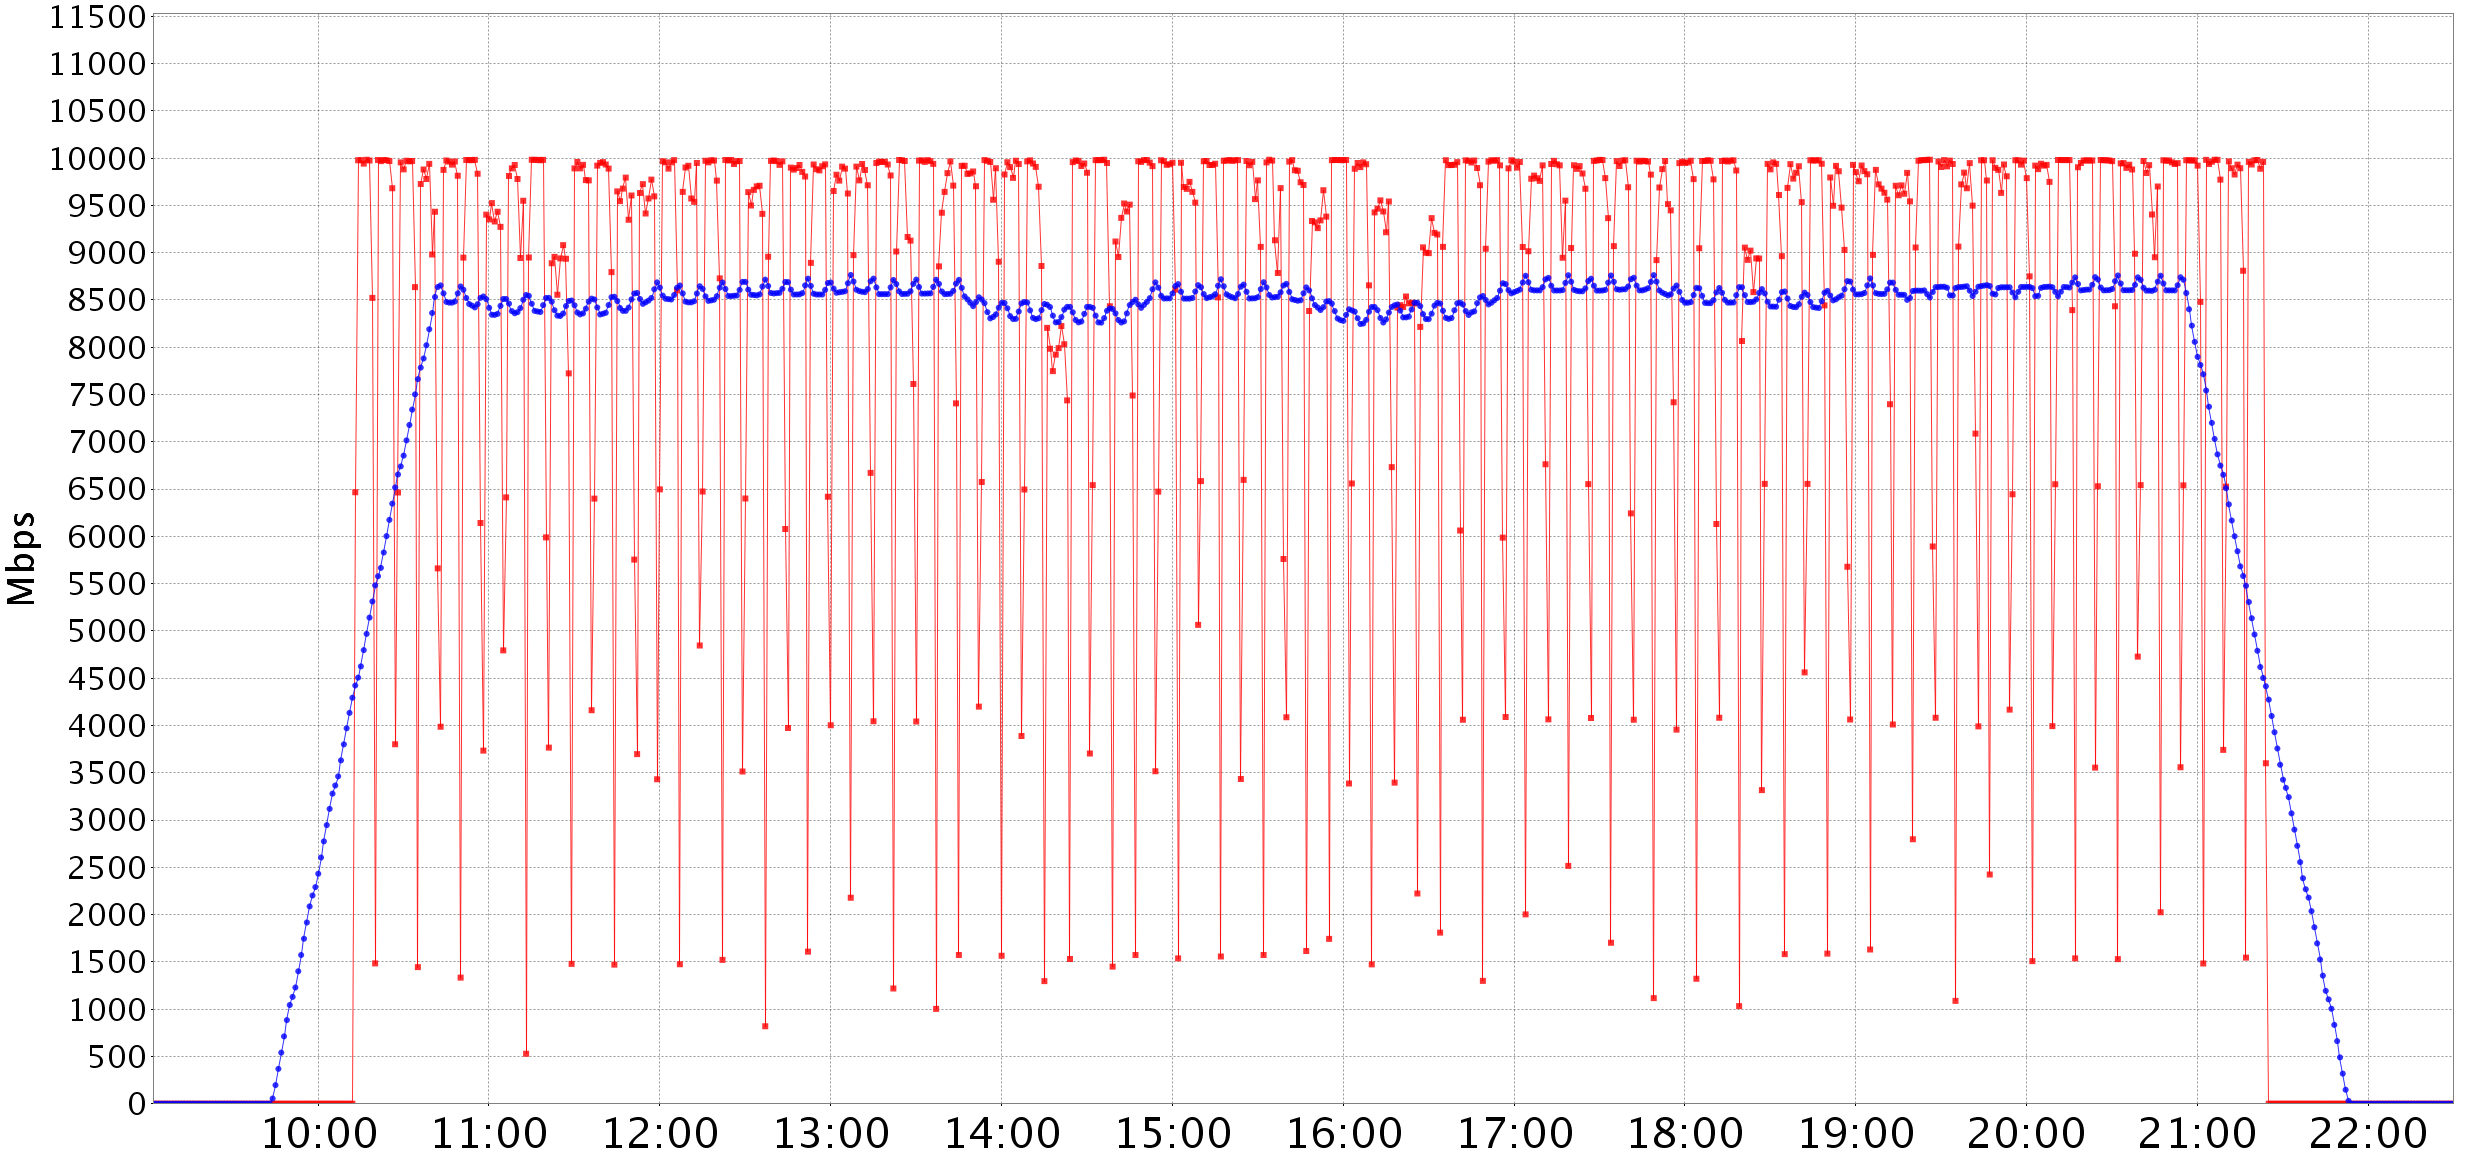
\includegraphics[width=0.95\textwidth]{FileDownload_Solo_path.png}
  \caption{PhEDEx transfers on the dedicated path}
    \label{fig:solo_transfers}
\end{figure} 

Figure \ref{fig:combined_transfers} and Figure \ref{fig:combined_phedex_transfers} show
the  network activity for PhEDEx traffic alone on both links. 
In this plot we can observe that PhEDEx switches to using the
new link without any interruption in service, doing it seamlessly and in a 
transparent way for the other instances (switch occurs around 10:00).

This plot also shows that there is a huge benefit to using the dedicated link.


\begin{figure}[h]
  \centering
  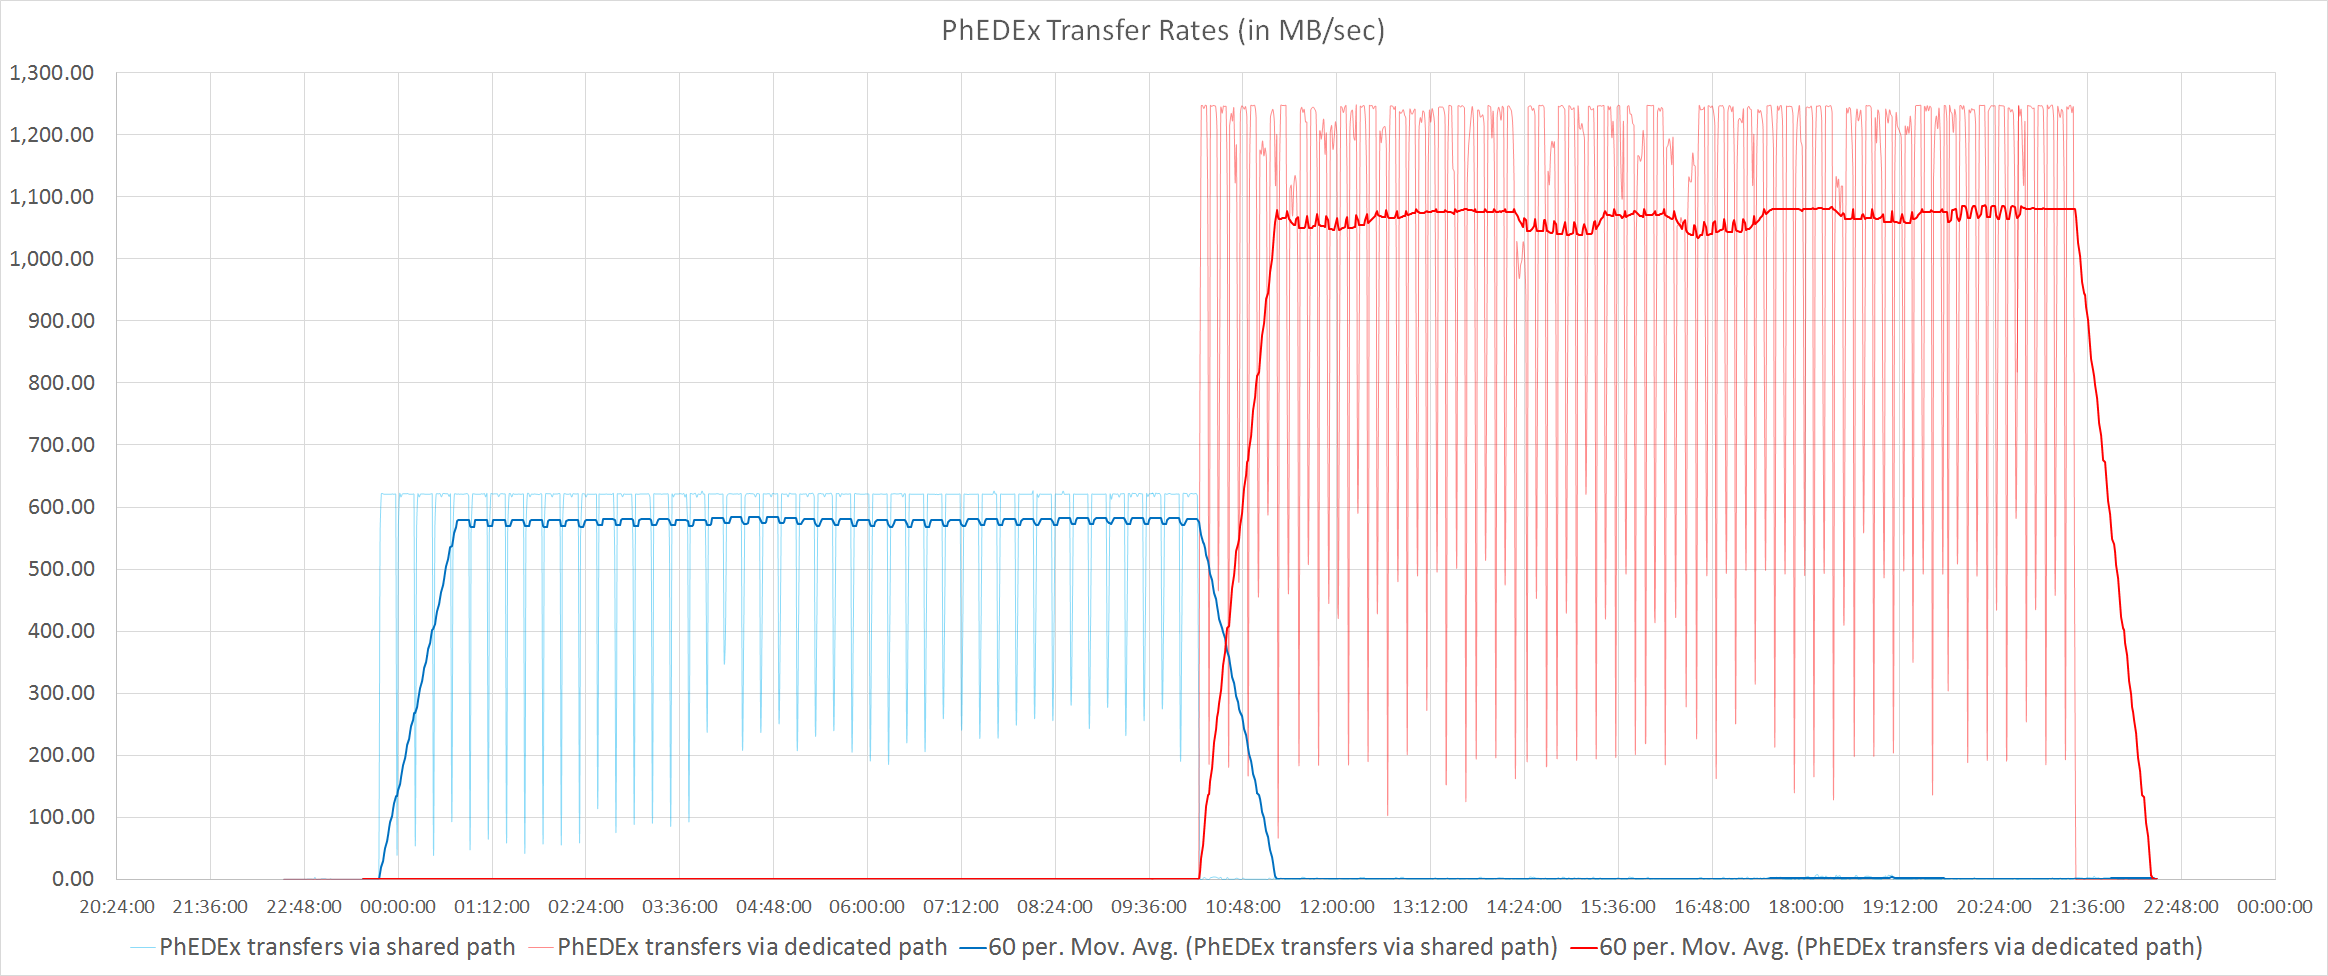
\includegraphics[width=0.95\textwidth]{FileDownload_All_paths.png}
  \caption{View of PhEDEx only transfers on both the shared and dedicated path}
  \label{fig:combined_transfers}
\end{figure} 

\begin{figure}[h]
  \centering
  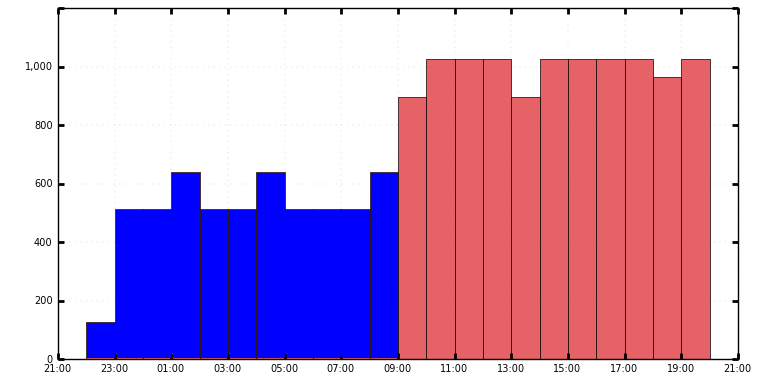
\includegraphics[width=0.95\textwidth]{FileDownload_PhEDEx_all_paths.png}
  \caption{View of PhEDEx only transfers on both the shared and dedicated path}
  \label{fig:combined_phedex_transfers}
\end{figure} 